\section{精度---承包人的观点}
\label{sec:4.7}

千里之堤,溃于一穴。一环薄弱,全局皆垮。经济的需要强迫所有的环节应该具珩相同
的强度。诸如与速度不确定性有关的误差,以及与叠后偏移有关而不是与叠前偏移有关的
误差等,有许多广泛性问题是值得研究的。对本书内容既然已经理解很多了,你现在有资格
去着手解玦这些广泛性问题。现在我们要缩小我们的注意范围,仅只考察向下延拓中由熟悉
的数据处理近似所产生的误差。

在波动方程偏移生产性程序的结构中,薄弱环节出现在许多不同地方所作的近似上。出
于节约的考虑,人们必须把周于提高资料精度的资金投资于该资金能获最佳经济效益之处。地
球物理承包商很自然就成了在叠加资料偏移方面对精度与费用进行权衡利弊的专家,承包商
将采用下面所收集的程序和一些方程,以最低的费用获得最佳的结果。使用反射资料的用户对
学会识别不完善的偏移一事会有兴趣,所以他们大概想利用该程序来看一下各种捷径的效果。

为重大生产任务作准备时,进行精度检查有两种一般性处理办法。第一种办法屉用各种
:方法作合成的双曲线,它给出关于定性现象的最透徹理解,可以用录像系统或者绘在幻灯片
上的方式将合成双曲线同手头的数据加以比较。在第二种处理办法中,你要按不同的网格大
小计算出波在不同时差和频率等等情形下的荻曲面或球面之旅行时间,然后可以执行一个最
优化方法的程序,使重要参数范围内的平均误差达到极小。

要想知道合成双曲面看起来像什么,没必要去写一个时间域45°有限差分偏移程序,我
们可以在$(\omega,k_x)$域内简单表示出所有公式,然后就作二维逆Fourier变换。为方便于在
许多种偏移方法之间进行比较,我们将按需要的先后顺序从本书的不同部分搜集各该方程。
到时我会提出可为许多种方法作出绕射双曲线的程序,采用相同的方程时,你就能计算出旅
冇时间并按你的希望解出最优化问题。

\subsection{横向导数}
\label{sec:4.7.1}

首先,$k_x$将变化于$\pm\frac{\pi}{\Delta}$的范围内。如果打算沿$x$轴作有限差分处理,这时我们将需要
有
\begin{equation}
(\frac{\hat{k}\Delta x}{2})^2=\frac{\sin^2\frac{k\Delta x}{2}}{1-b4\sin^2\frac{k\Delta x}{2}}
\label{eq:ex4.3.7b}
\end{equation}
所以,如x轴准备按有限差分处理,则以后有关$k_x$的项都应当用$\hat{k_x}$代替。进行有限差分时,
引入了自由参量b,类似地,你也可以用一个接近于1的可调参量来标定整个表达式。还有,
$\Delta x$没必要受数据采集的限制而固定死,你总是能够在处理之前对数据进行内插的,有足够
的横向速度变动就得强制有限差分方法采用经过内插的数据。

\subsection{粘滞性与因果性}
\label{sec:4.7.2}


频率将变化于士疋/Af的范围内,如果打算沿f轴作有限碧分处理,这时我们将需要Z变换变量
\begin{equation}
Z=e^{i\omega \Delta t}
\label{eq:ex4.6.2}
\end{equation}
以及服从因果律的导数
\begin{equation}
-i\hat{\omega}=\frac{2}{\Delta t}\frac{1-\rho Z}{1+\rho Z} \quad \quad -1\leq \rho <1
\label{eq:ex4.6.29}
\end{equation}
在处理之前,数据可能是采样不足或过采样的,所以$\Delta t$应该是一个可補参量。因杲性参量$\rho$
应是小于1的数,比方说,$\rho =1-\epsilon$,此处$\epsilon>0$是一可调参量。即使你在频率域内进行偏移,
你也许还是需要引入$\rho$,因为它可减小时间域内出现的折叠现象一这是粘滞性的一种类
型。$\epsilon$应大致等于数据长度的倒数$1/N_t$,此处$N_t$,是时间轴上的采样点数(因为我曾以平方根
増益$\gamma= 1/2$作过许多合成双肋线的图形,时间域折叠现象都比实际的要严重一些,所以我已
经使程序中$\epsilon$的缺省范围大了四倍)。你如喜欢调节自由参量,那你可分别调节分母和分子
的$\rho$值。往后,我对$\omega$与$\hat{\omega}$将加以区别,但是你如不关心因果性的引入,你就可令$\hat{\omega}$为
$\omega$。

\subsection{Muir延迟递归}
\label{sec:4.7.3}

$k_z$的平方根可以用你计算机内的平方根函数或采用Muir展开的办法计算出来。为使
Fourier变换域的计算体现出因果性,你必须利用某种复值平方根函数,这样作也会自动地
照顾到耗散区---你不再有耗散区与非耗散区之间的不连续性了。复数的平方根是多值的,
所以你最好首先检查一下你的计算机是否选取了如图\ref{fig:crft/kzplane}中所示的相位。我就是曾经这样
作的,但是我发现,一直到我把表达式$\sqrt{s^2+v^2k^2}-s$用代数上与它等值的表达式
$v^2k^2/(\sqrt{s^2+v^2k^2}+s)$代替之前,受限制的数值精度总是妨碍了我使阻抗的实部达到严格的正值
性。

为进行有限差分,我们需要的将是Muir递归。设$r_0$定义为开始Muir递归时之角度的余
弦,这角度往往为0°或45°。对最优化来说,这个角度是另一个自由参量。例如可参见图
\ref{fig:omx/disper}。这种角度也是一个对所有阶次递归都准确拟合的角度。令
\begin{equation}
s=-i\hat{\omega}
\label{eq:ex4.6.29}
\end{equation}
从$R_0=r_0s$开始的Muir递归为
\begin{equation}
R_{n+1}=s+\frac{v^2k_x^2}{s+R_n}
\label{eq:4.6.30}
\end{equation}


对于绕射程序,我们将要对$\exp(-Rz)$进行计算。由于在\ref{sec:4.6}节中已证明$R$具有正实部,
该指数项应永不增长。存限差分计算通常是利用延迟时间完成的,为使时间有延迟,将$\exp(-Rz)$
表示为
\begin{equation}
e^{-Rz/v}=e^{-(R-s)z/v}e^{-sz/v}
\label{eq:4.7.1}
\end{equation}
正如\ref{sec:4.1}节中所讨论的,你大概并不想使延迟的时移与牯滞影响有联系,所以你大概会想使
向下延拓用下式代替
\begin{equation}
e^{-[R(-i\hat{\omega})+i\hat{\omega}]z/v}e^{+i\omega z/v}
\label{eq:ex4.7.2}
\end{equation}
注意其中的符号和$\omega$有别于$\hat{\omega}$。

由式\ref{eq:4.6.30},我们知道$R-s$应具有一正实部。我曾发现数值舍入有时会妨碍这点,
所以曾将Muir递归重新加以组织,使之体现出延迟作用。令
\begin{equation}
R'=R-s
\label{eq:ex4.7.3}
\end{equation}
式(4.6.30)变为
\begin{equation}
R_{n+1}'=\frac{v^2k_x^2}{2s+R_n'}
\label{eq:ex4.7.4}
\end{equation}
根据Muir规则,你能看出,如果我们按这种途径开始递归,就会总是具有正实部。所以
我们就由下式开始递归
\begin{equation}
R_1'=\frac{v^2k_x^2}{s(1+r_0)}
\label{eq:ex4.7.5}
\end{equation}
(把式\ref{eq:ex4.7.5}与式\ref{eq:ex4.7.3}结合起来就可得出如式\ref{eq:4.6.30}给出的相同15°方程)。
从数学上说,式\ref{eq:ex4.7.2}恒等于下式
\begin{equation}
e^{-R'x/v}e^{+i\omega z/v}
\label{eq:ex4.7.6}
\end{equation}
但是在数值上式\ref{eq:ex4.7.6}中的指数沿z方向衰减是有保证的。

\subsection{沿深度步进}
\label{sec:4.7.4}

如果你沿深度或者旅行时间深度采用有限差分,那么我们就有下列关系:
\begin{equation*}
\frac{\hat{k_z}\Delta z}{2}=\tan\frac{k_z\Delta z}{2}
\end{equation*}
此式可应用于$\exp ik_zz$。由于可能存在耗散,上述各董可以是复数。令$N_z$为沿深度的层数,
一般而言它能等于或小于$N_t$。使式\ref{eq:ex4.3.17}适用于式\ref{eq:ex4.7.6},得出
\begin{equation}
e^{-R'N\Delta z/v}\approx (\frac{1-R'\Delta z/2v}{1+R'\Delta z/2v})^N
\label{eq:ex4.7.7}
\end{equation}

\subsection{闪电式的相移偏移}
\label{sec:4.7.5}

不仅能使时间域方法的因果性与粘滞性特征在频率域内体现出来,而且相移方法的平方
根和复指数也能用复数乘法与除法来代替。首先要注意,平方根展开并不需要从某个起始猜
测开始或从某个低阶叠代过程开始,它能够从以前由前面的$\omega$或k所预先得出的平方根开始。
(我注意到这点可以说是歪打正着,那时程序的早期飯本曾有一处毛病,使我所有的15°偏
移计算都看起来像是90°偏移计算结果)。还有,在相移法中的$\Delta z/v$要小到必要的程度,以
适应在每个时间点上的成像。所以,按式\ref{eq:ex4.7.7}形式进行有限差分大概同采用复指数形
式时一样效果良好,你不妨试它一试。

\subsection{最终显示面貌}
\label{sec:4.7.6}

脉冲响应程序的输出总是很糟糕,主要原因在于$(\omega,k_x)$空间中的很大面积是位于
Nyquist频率附近或者位于倏逝波截止带以上。由于我们很少可能按Nyquist准则所允许的
稠密程度沿时间对数据进行采样,下面给出的程序将缺省以滤波因子$(l + Z)/( 1
-0.8Z)$
进行的最终滤波处理,在地震资料通常频带范围之外的大量能量仍然能通过这种滤波。因为
所有陆地资料和大多数海上资料都没有零频率分量,所以该程序包含了进一步采用$(1
-Z)(1-0.8Z)$的可供选择的滤波。我一直没采用这科额外的滤波来显示过任何东西,因为我
想使本书反映出所有你也许会碰见的假象。另外,我采用\ref{sec:4.1}节所述非线性増益$\gamma=1/2$时,
有意地在波形曲线、变面积记录图形上増强了各种假象的可见度(透视图屏蔽线总是具有线
性增益)。由于我的图形在本书中大约为10公分见方,而你在实际工作中将看到的图形大约
为这种面积的100倍,所以我仅显示了1秒的旅行时间。



\subsection{程序}
\label{sec:4.7.7}

书中许多图许都是用这里提出的程序作出来的,为使你能够重新产生它们,我在下面列
出了完整的程序。参量输入与数据输出的调用均由地址决定,但是我使它们无论以何种方式
都能有劢于澄清缺省项,使你有可能获得与我所曾得出的是完全相同的结果

\begin{figure}[H]
\centering
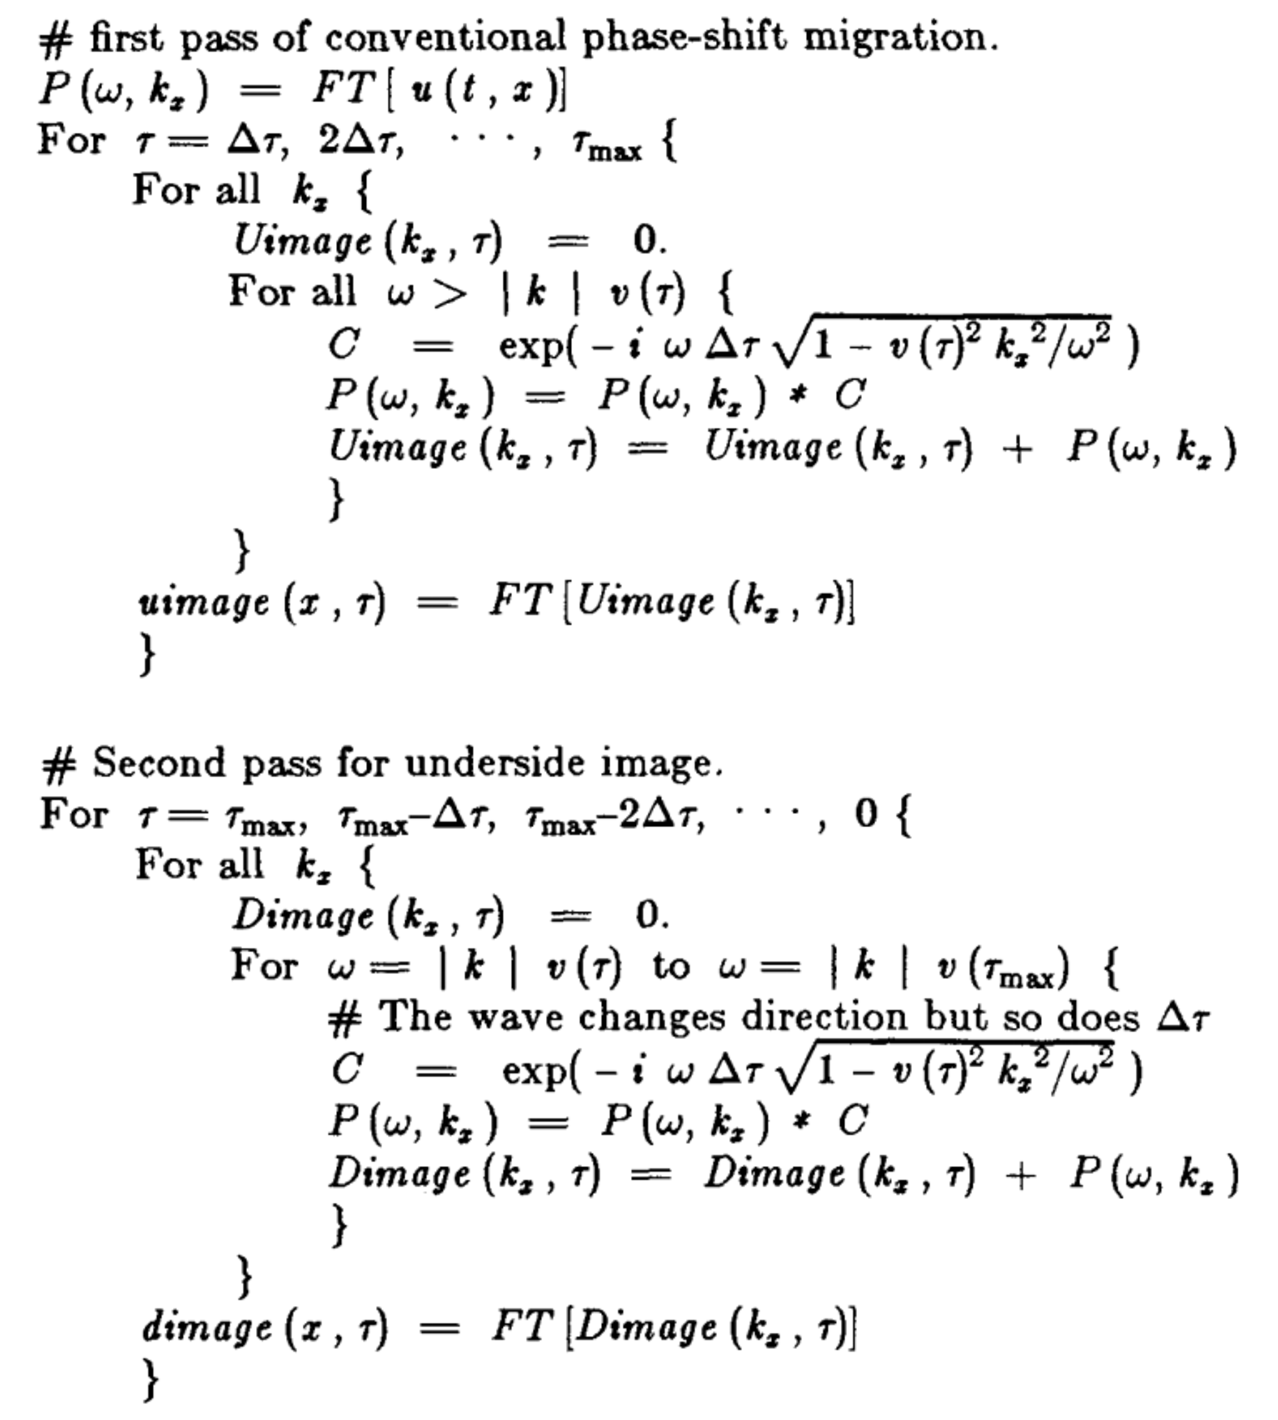
\includegraphics[width=0.65\textwidth]{crft/code1}
\label{fig:crft/code1}
\end{figure}
\begin{figure}[H]
\centering
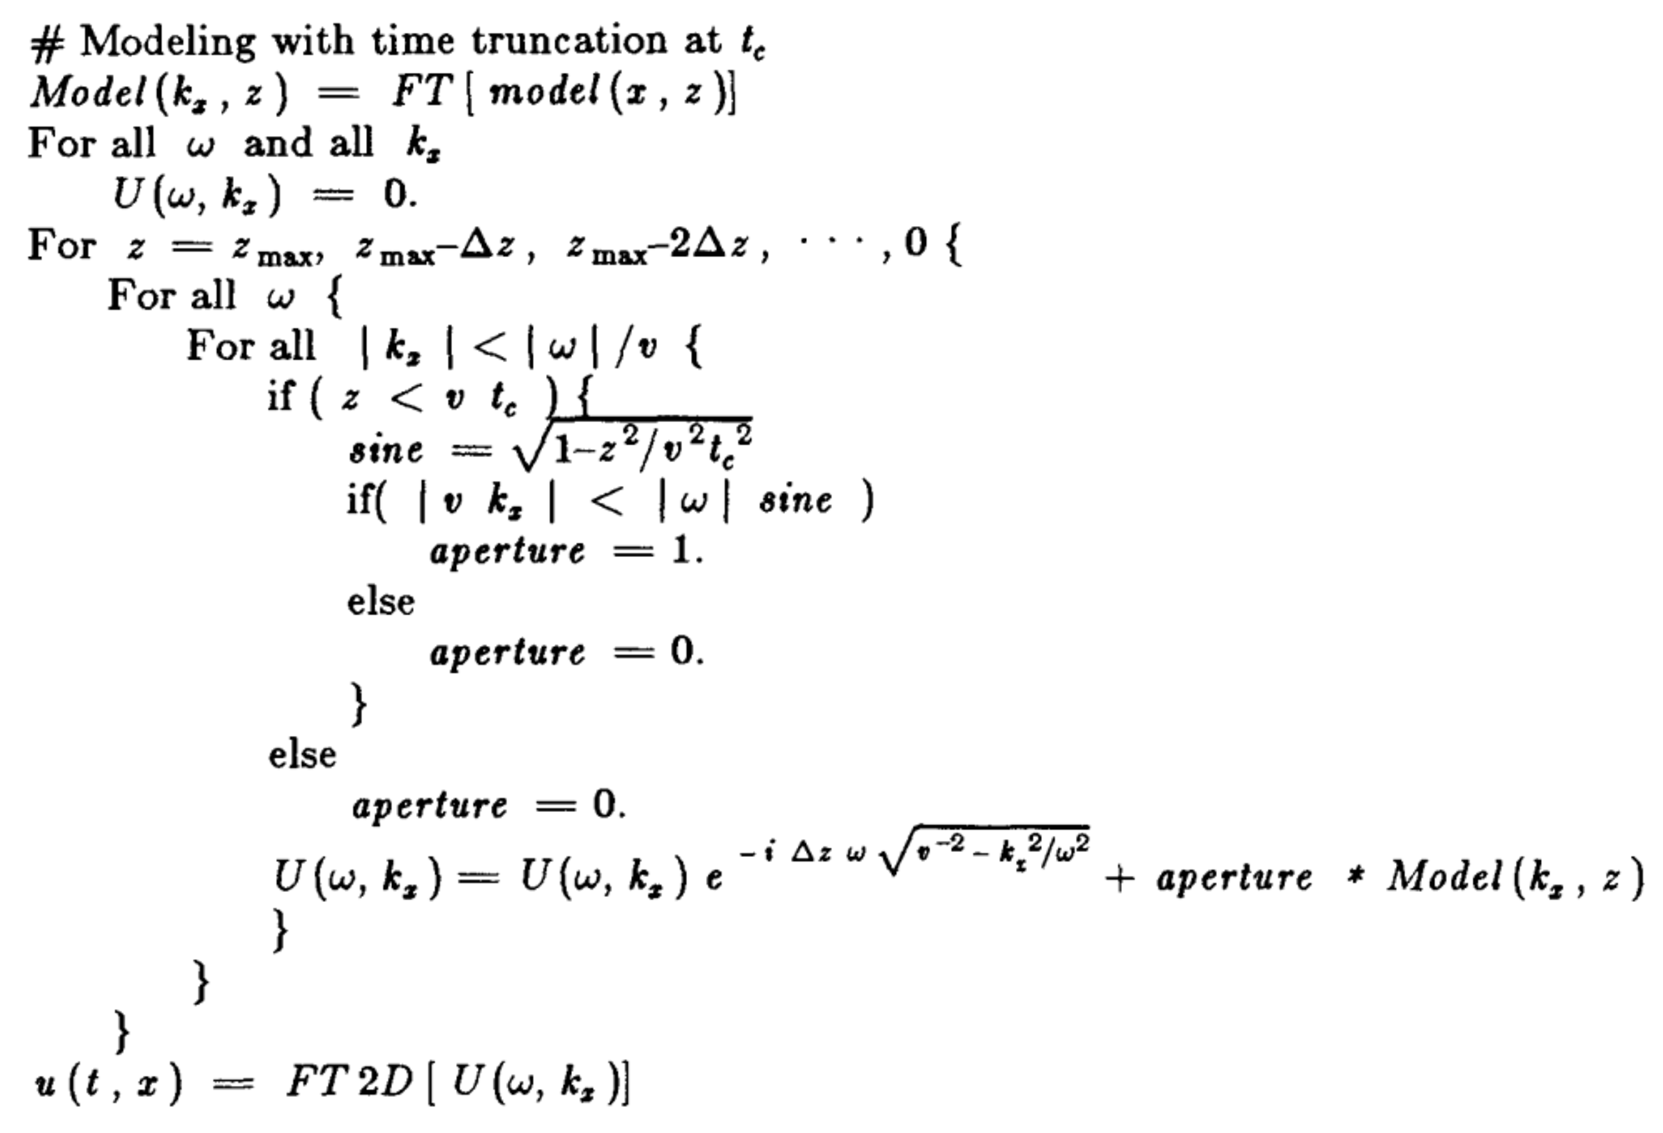
\includegraphics[width=0.65\textwidth]{crft/code2}
\label{fig:crft/code2}
\end{figure}
\begin{figure}[H]
\centering
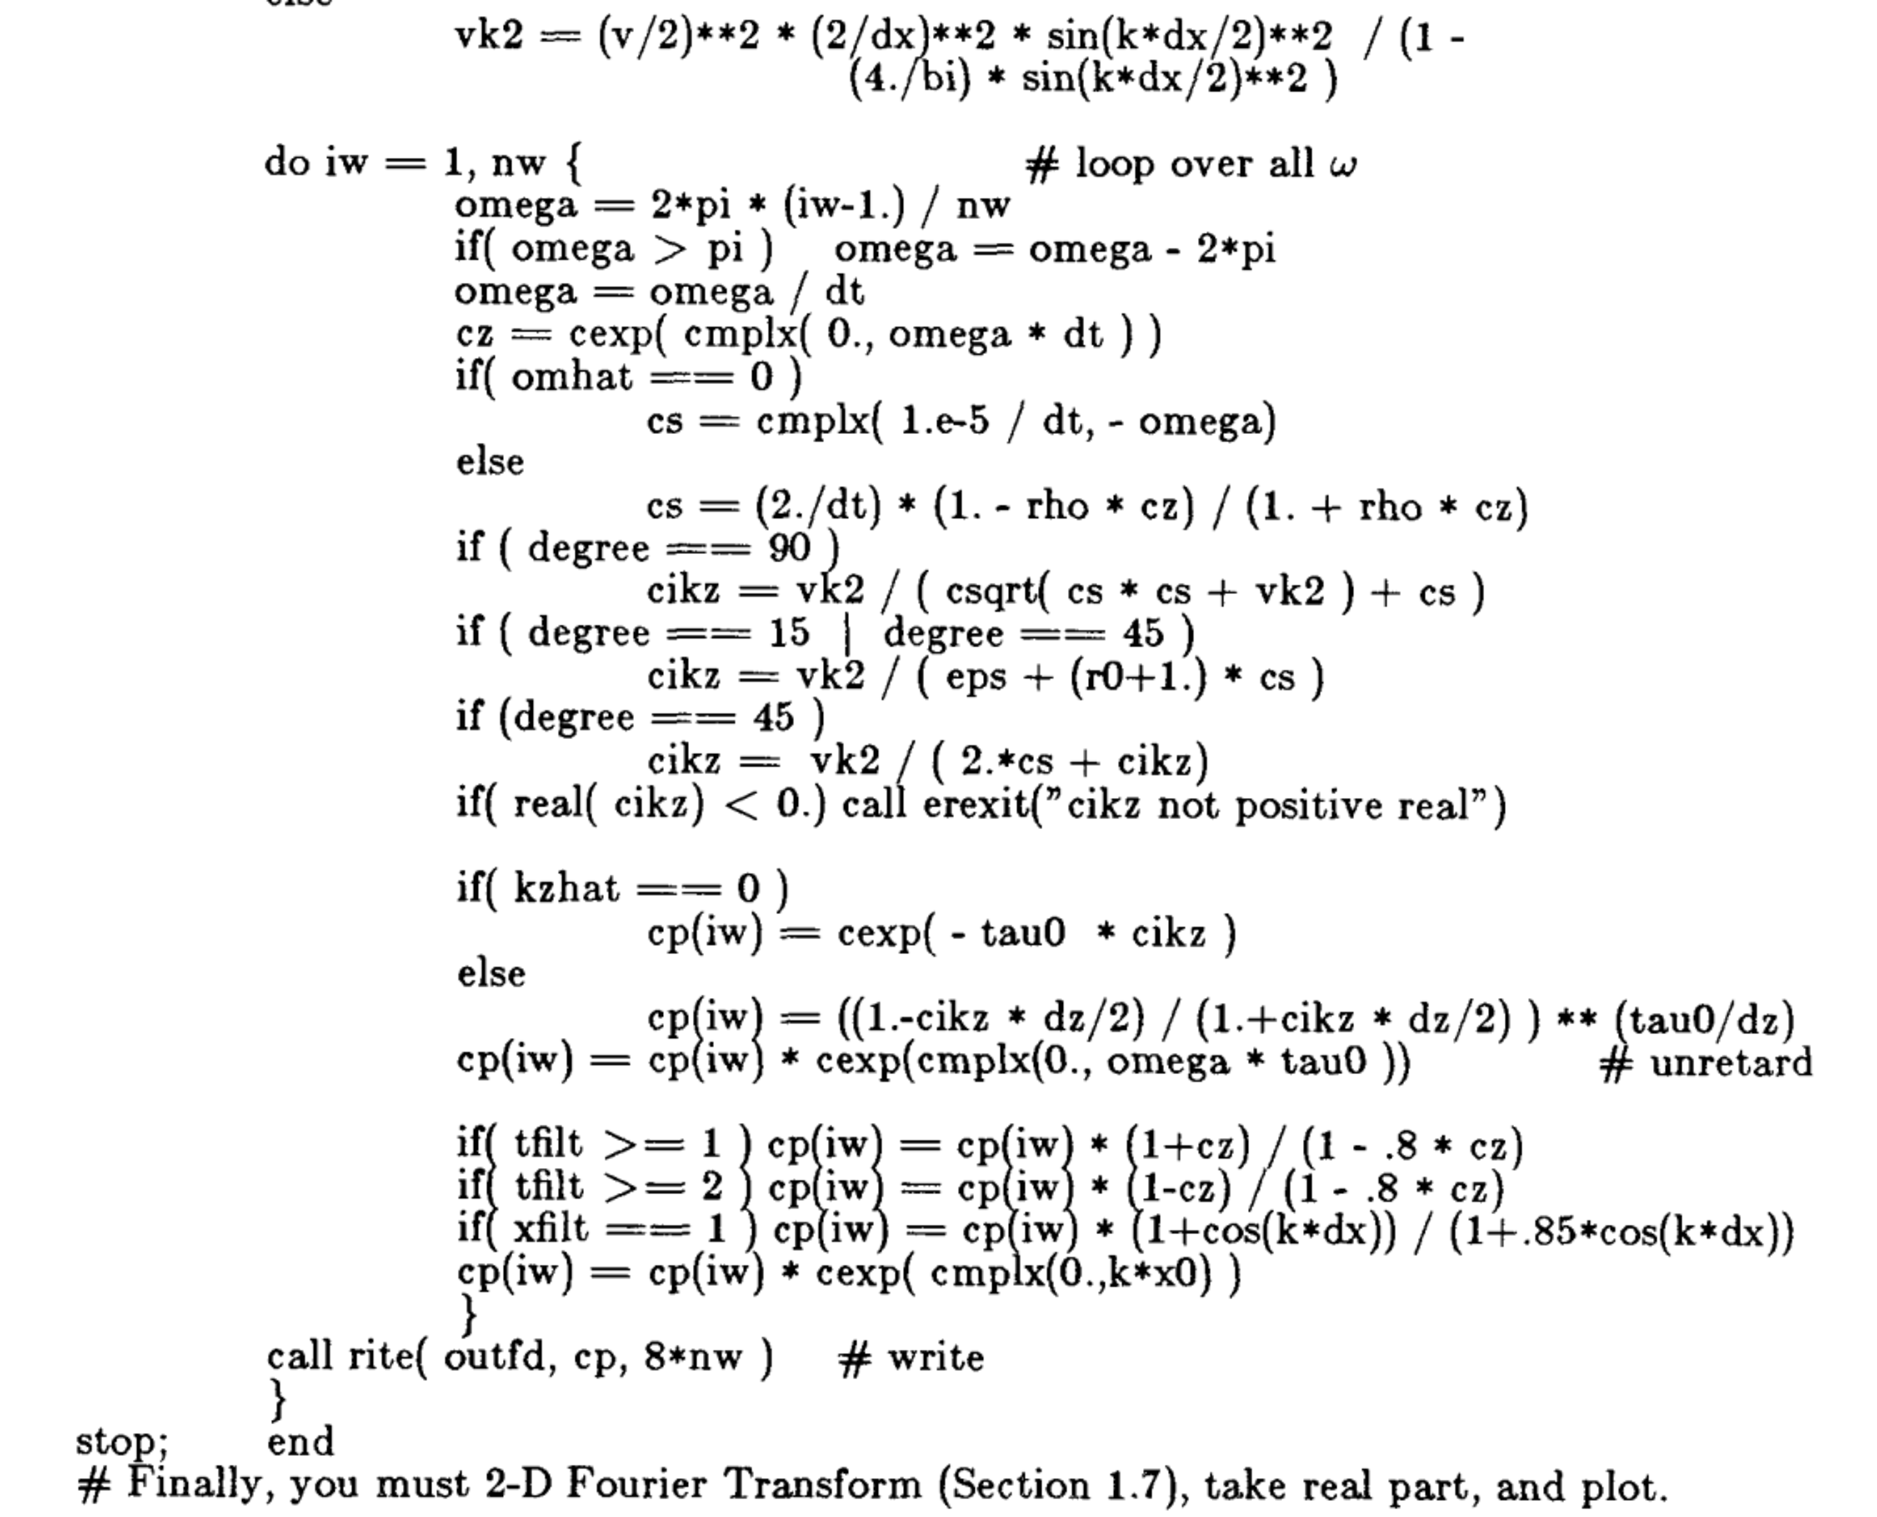
\includegraphics[width=0.65\textwidth]{crft/code3}
\label{fig:crft/code3}
\end{figure}

本书内有22个图件是由这个程序作出的,不同图件所采用的不同输入参量列表如下:
\begin{table}[!ht]
\centering
\ttfamily
\small
\begin{tabularx}{\textwidth}{|Y|Y|}
\hline
节号与图号 & 缺省参量 \\
\hline
1.3-6a & tfilt=0 \\
\hline
1.3-6b & \\
\hline
2.0-1a & \\
\hline
2.0-1b & $\hat{\omega}$ \\
\hline
4.0-1a & $\hat{\omega},v=2.0, xf=.5, xfilt=0$ \\
\hline
4.0-1b & $\hat{\omega},v=2.0, xf=.5 $ \\
\hline
4.1-4a & 15°\\
\hline
4.1-4b & $15^{\circ},\epsilon=1$\\
\hline
4.1-5a & $45^{\circ},tf=.2$\\
\hline
4.1-5b & $45^\circ, tf=.2, \epsilon=1$ \\
\hline
4.2-4 & $45^\circ, tf=.2, \hat{\omega}$\\
\hline
4.3-4a & $v=2.0,90^\circ$\\
\hline
4.3-4b & $v=2.0,15^{\circ},\hat{\omega},\hat{k_x},\hat{k_z}$\\
\hline
4.3-6a & $\hat{k_x},\hat{\omega},b^{-1}=1000000.$\\
\hline
4.3-6b & $\hat{k_x},\hat{\omega},b^{-1}=12.$\\
\hline
4.3-6c & $\hat{k_x},\hat{\omega},b^{-1}=6.726$\\
\hline
4.3-6d & $\hat{k_x},\hat{\omega},b^{-1}=6.$\\
\hline
4.3-6e & $\hat{k_x},\hat{\omega},b^{-1}=5.$\\
\hline
4.6-2a & \\
\hline
4.6-2b & $\hat{\omega}$ \\
\hline
4.7-1a & $\Delta z=.004,45^{\circ},tf=.3,\hat{\omega},\hat{k_x},\hat{k_z}$\\
\hline
4.7-1b & $\Delta z=.012,45^{\circ},tf=.3,\hat{\omega},\hat{k_x},\hat{k_z}$\\
\hline
\end{tabularx}
\end{table} 

据说使z网格加密就能改善精度,如果x与t均属于连续统(continuum
)这种结果是不
可能发生的,不过由于可使x与t离散化,偶然能消掉误差的可能性倒是存在的。为检查一下
这种传说是否成立,我试着把$\Delta z$増大3倍(实际上,就是将沿旅行时间深度的增量増大
3倍),结果如图\ref{fig:dspr/bigdz}所示。你对这图有何想法?

\begin{figure}[H]
\centering
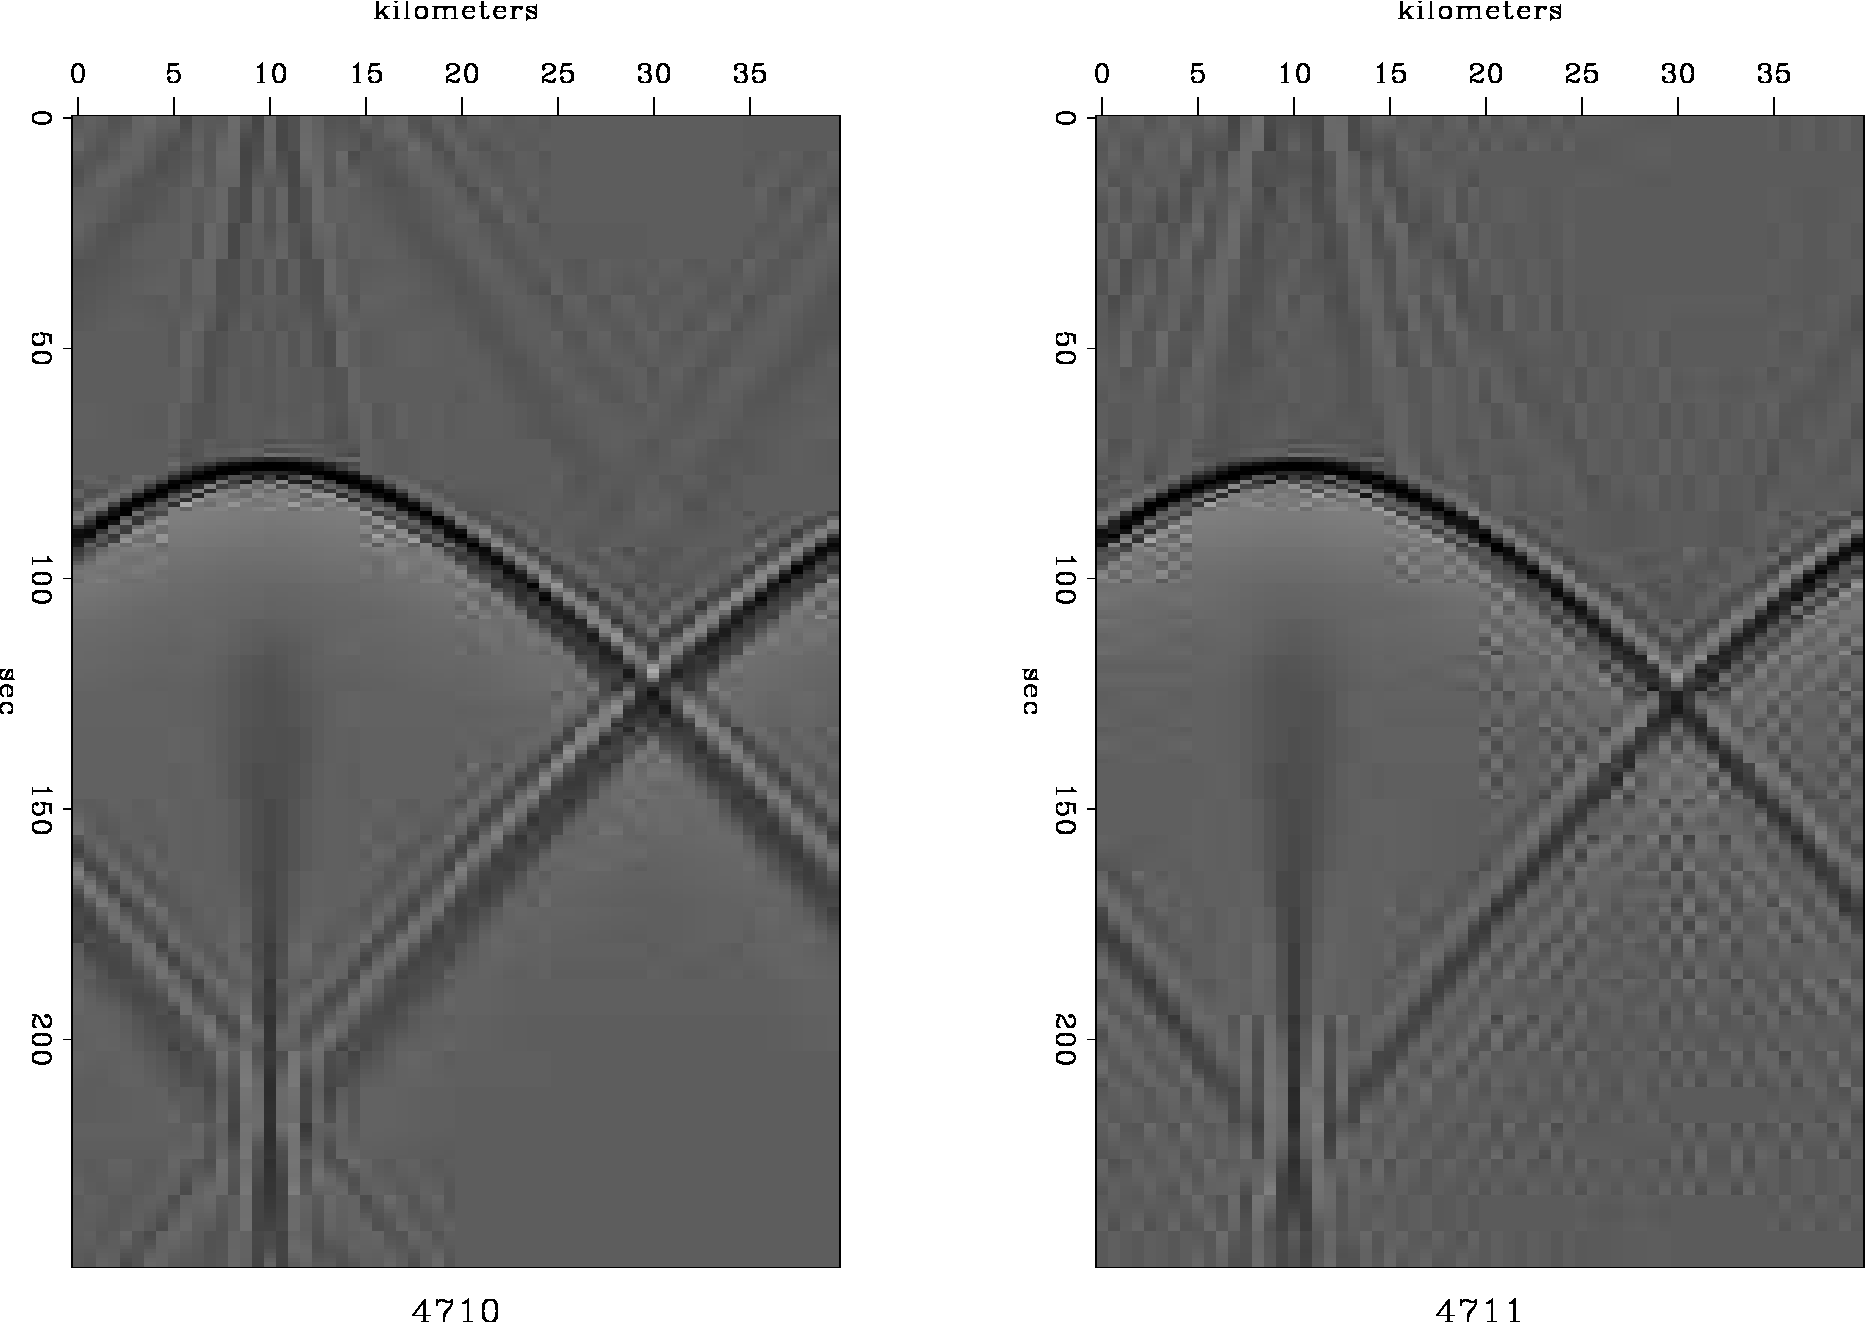
\includegraphics[width=0.65\textwidth]{dspr/bigdz}
\caption[bigdz]{$(x,z,t)$空间中的45°点绕射,左图为$\Delta z=v\Delta t$,右图为$\Delta z=3v\Delta t$}
\label{fig:dspr/bigdz}
\end{figure}

这种分析看来就得到此结束了,由于Fourier分析是假设速度横向为恒定不变,分析受
到了限制。为处理这种问题,我们现在就转向下面一节有关处理技术这最后一讲。
